\section{次元圧縮が与える影響の評価実験}
本研究では,ユーザ-アイテム行列を直接重回帰分析する場合(直接法)と,圧縮空間で重回帰分析を経て元の次元のパラメータを推定する場合(提案法)の予測精度を求める.
また,直接法と提案法により得られたパラメータについて,その差異を検証する.
併せて,ユーザ-アイテム行列の重回帰分析にL1正則化(lasso)とL2正則化(ridge)を適用した場合についても比較する.

\subsection{実験環境}
本実験では,Book-Crossingデータセットを用いる.
このデータセットは,ユーザが書籍に付与した1から10までの10段階のスコアを集計したものであり,ユーザ数278,858,書籍数271,379,総スコア数383,852である.

予測精度の検証には,ユーザ-アイテム行列を直接重回帰分析する必要がある.
データの全書籍を説明変数とすると,観測データ数が足りず重回帰分析のパラメータ推定ができない可能性があるため,評価しているユーザの多い書籍上位$n+1$件を変数として選択し,選択した変数のスコアデータのみを用いる.
$n+1$件の変数から目的変数をひとつ選択し,残りの$n$件を説明変数とする.
本実験では,説明変数の数$n$は20から100まで10ずつ増やしていく.
選択したすべての変数をそれぞれ目的変数として設定し,目的変数毎に回帰式を立てる.
なお,説明変数に含まれる欠損値は,スコアの中央値である5.5で補完することとする.

線形写像$\boldsymbol{W}$を得るためのword2vecのハイパーパラメータは,次元数$k=10$,学習の最大単語数100,ネガティブサンプリング数5,トレーニング反復回数500,最小出現数0,Skip-gram学習モデルとしている.


\begin{figure*}[t]
  \centering
    \begin{tabular}{ccc}
           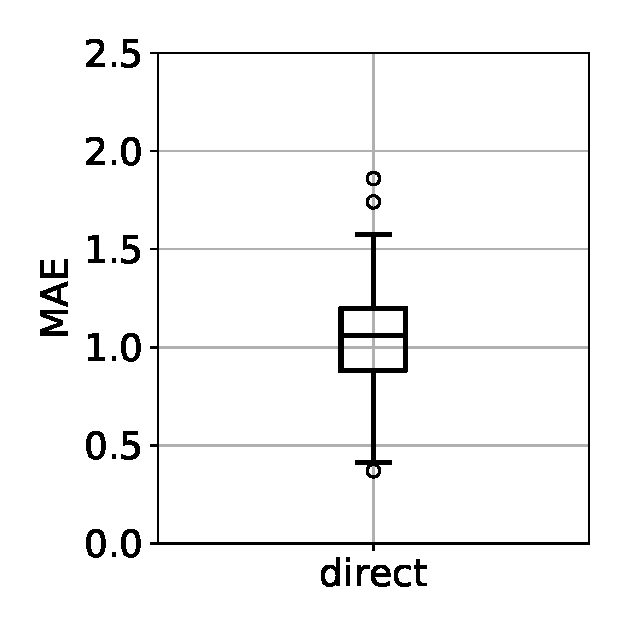
\includegraphics[width=0.25\hsize]{img/direct-mae-lasso.eps} &
           \includegraphics[width=0.30\hsize]{img/lasso-2.eps} &
           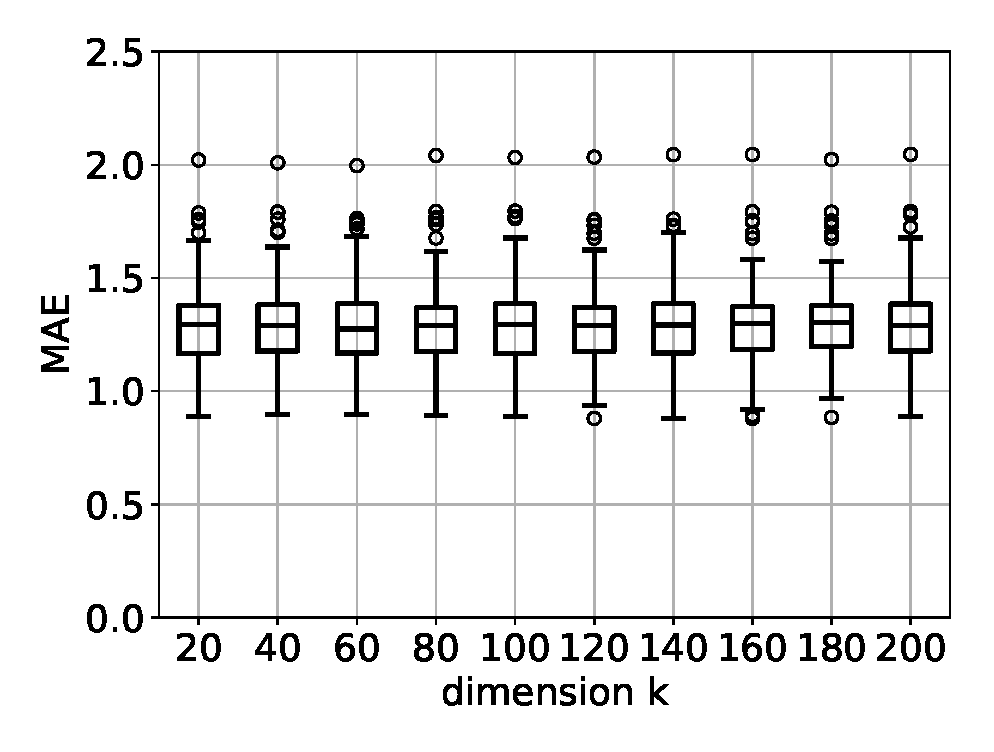
\includegraphics[width=0.30\hsize]{img/lasso-10.eps} \\
           \small  (a) 正則化法& \small  (b) 次元圧縮法(ウィンドウサイズ2) & \small  (c) 次元圧縮法(ウィンドウサイズ10) \\
    \end{tabular}
        \caption{L1正則化を適用した正則化法と次元圧縮法のスコア予測精度}
    \label{lasso}
%  \end{center}
\end{figure*}

\begin{figure}[t]
  \centering
           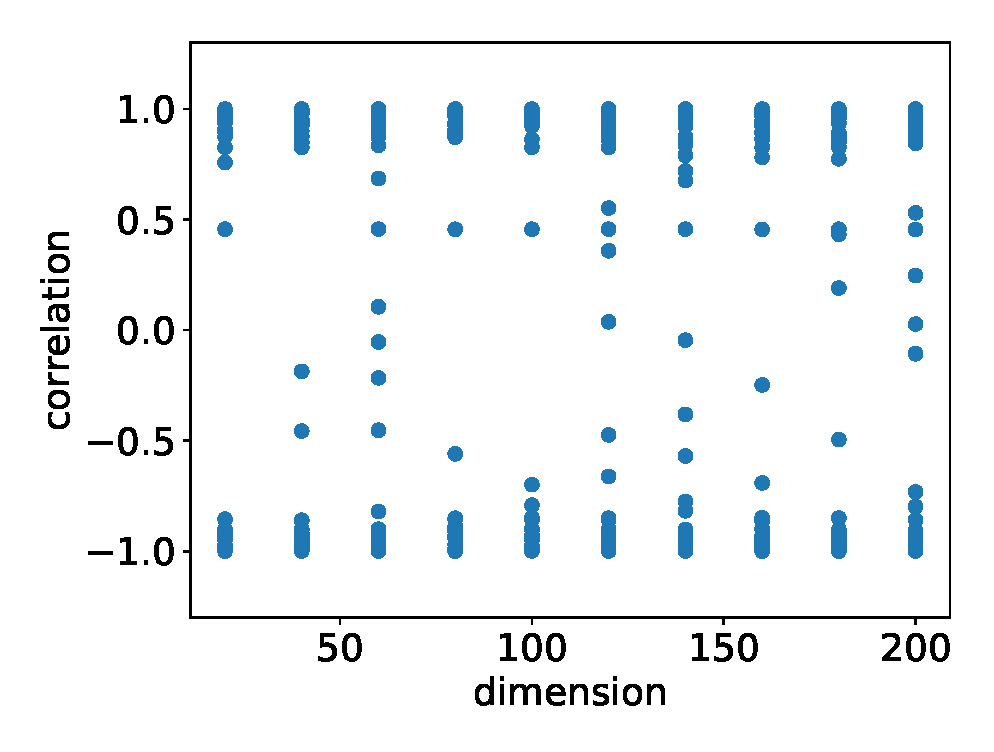
\includegraphics[width=0.8\hsize]{img/lasso-correlation-2.eps} \\
           \small ウィンドウサイズ2
        \caption{正則化法と次元圧縮法の偏回帰係数の相関(L1正則化)}
    \label{soukan}
%  \end{center}
\end{figure}
\begin{table}[t]
\begin{center}
\caption{正則化法と次元圧縮法のモデルの学習時間[s]}
  \begin{tabular}{c|c|cccc|c} \hline
      & \small 正則化法 & 次元圧縮法 \\ \hline
     \small L1正則化 & 34.2 & 23.6 \\
     \small L2正則化 & 77.4 & 23.4 \\  \hline
      \end{tabular}
      \label{jikkou}
      \end{center}
\end{table}

\subsection{予測精度の比較と考察}
本実験では,予測精度として平均絶対誤差(MAE: Mean Absolute Error)$MAE = \frac{1}{N} \sum_{i=1}^N |\hat{y_i} - y_i|$を用いる.
$N$はテスト用データ数,$\hat{y_i}$は予測値,$y_i$は真値とする.
MAEは値が小さいほど予測精度が良いという指標である.

図\ref{fig:result1}に,$n=50$までの直接法と提案法の予測精度の箱ひげ図を示す.
縦軸はMAEの値,横軸は説明変数の数を表している.
$n=20$においては,直接法と提案法の予測精度に違いがないことがわかる.
また,図\ref{fig:result1}(a)より,直接法は目的変数の数が増えるに従ってMAEも大きくなり,予測精度が悪くなっている.
目的変数の数に対して観測データが足りなかったためと考える.
一方で,図\ref{fig:result1}(b)より,提案法の予測精度は目的変数の数に影響されないことがわかる.
そのため,直接法では重回帰分析できない場合でも提案法は適用できると考える.

図\ref{fig:result2}に,直接法(direct)と提案法(proposal)それぞれにL1正則化(lasso)およびL2正則化(ridge)を適用した際の予測精度の箱ひげ図を示す.
図\ref{fig:result2}より,提案法に正則化を適用した場合と正則化を適用しない場合の予測精度は,MAEの中央値で0.05程度の差しかないことがわかる.
また,提案法に正則化を適用しない場合と直接法に正則化を適用した場合の予測精度も,同様にMAEの中央値で0.05程度の差しかない.
そのため,提案法は直接法に正則化を適用したときと同様の結果を得られると考える.

\subsection{推定したパラメータの比較と考察}
図\ref{fig:result3}に,提案法で得られたパラメータについて直接法で得られたパラメータ,直接法にL1正則化(lasso)およびL2正則化(ridge)を適用したときのパラメータ
との相関係数の箱ひげ図を示す.
重回帰分析では,推定したパラメータから目的のアイテムに影響を与える他のアイテムを調べることができる.
相関係数が高いほど推定したパラメータの値が似ている傾向にある.
図\ref{fig:result3}より,提案法と直接法にL2正則化(ridge)を適用した場合のパラメータの相関係数の中央値が高く,ばらつきが非常に小さいことがわかる.
これより,提案法は直接法にL2正則化(ridge)を適用したときと同様の効果があると考える.